\documentclass[12pt]{article}
\usepackage[T1]{fontenc}
\usepackage{graphicx}
\usepackage{caption}
\usepackage{array}
\title{Systemy Wbudowane\\
   Projekt\\
   Schemat komponentów i połączeń}
\author{Piotr Popis}
\date{Maj 2020}

\begin{document}

\begin{titlepage}
\maketitle
\end{titlepage}

\section{Schemat Komponentów}
\subsection{Kolor sensor TCS3200}
\begin{center}
\begin{minipage}[H]{.45\textwidth}
    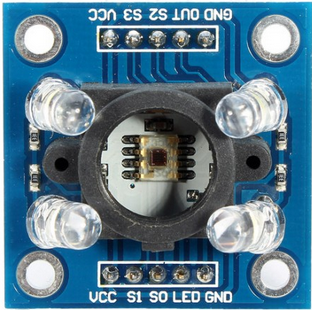
\includegraphics[width=.8\linewidth]{tcs.png}
\end{minipage}
\end{center}
\subsubsection{Opis}
Sensor jest odpowiedzialny za odczyt( wykrycie) koloru obiektu.\\
\\
Umożliwia konwersje natężenia światła do częstotliwości RGB
 ( Light    intensity -> frequency). Na jego wyjściu mamy częstotliwości dla danego koloru. Czujnik jest kompatybilny z Arduino. 
\subsubsection{Specyfikacja}
\begin{center}
\begin{tabular}{ | m{5cm} | m{3cm} | } 
\hline
Napięcie &  2.7- 5.5V\\ 
\hline
\multicolumn{2}{|c|}{Bezpośrednio komunikuje się z Mikrokontrollerem}\\ 
\hline
\multicolumn{2}{|c|}{Konwersja światła o wysokiej rozdzielczości na częstotliwość}\\ 
\hline
\multicolumn{2}{|c|}{Funkcja wyłączania}\\ 
\hline
\multicolumn{2}{|c|}{Programowalny kolor i częstotliwość wyjściowa w pełnej skali}\\ 
\hline
\end{tabular}
\end{center}
Posiada cztery rodzaje filtrowania:\\
\begin{minipage}[H]{.5\textwidth}
    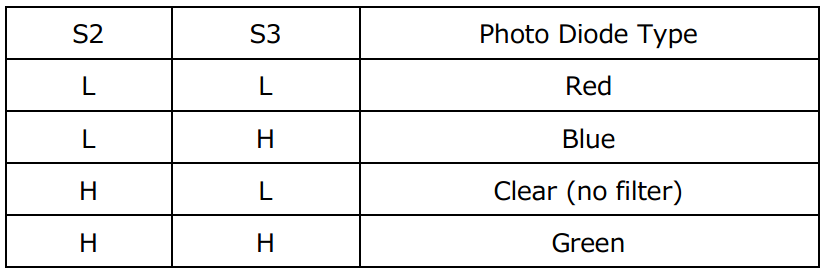
\includegraphics[width=1.8\linewidth]{filtry.png}
\end{minipage}
\subsection{Serwo micro servo SG90 Tower Pro}
\begin{center}
\begin{minipage}[H]{.85\textwidth}
    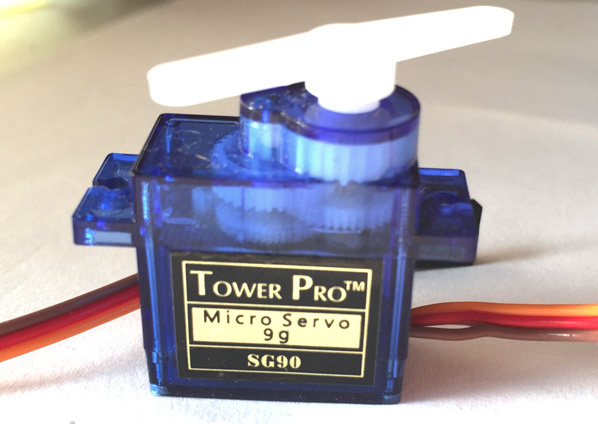
\includegraphics[width=1.0\linewidth]{serwo.png}
\end{minipage}
\end{center}
\subsubsection{Opis}
W systemie wykorzystywane są dwa serwa: górne i dolne. Serwo górne ma dwa zadania do wykonania podawanie obiektu z wejścia pod sensor i zepchnięcie spod senora na zsuw. Natomiast serwo dolne ustawia zsuw pod odpowiednim kątem.
\subsubsection{Specyfikacja}
\begin{center}
\begin{tabular}{ | m{5cm} | m{3cm} | } 
\hline
Napięcie &  4.8 V (~5V)\\ 
\hline
Moment przegięcia & 0.1 s/60º\\ 
\hline
Szybkość operowania & 1.8 kgf·cm\\ 
\hline
Szerokość strefy nieczułości & 10 µs \\ 
\hline
Zasięg temperatury &  0 ºC – 55 ºC  \\ 
\hline
Zasięg obrotu &  180º  \\ 
\hline
Waga &  9 g  \\ 
\hline
Wysokość & 27 mm\\
\hline
Szerokość & 22 mm\\
\hline
Głębokość & 11,5 mm\\
\hline
\end{tabular}
\end{center}

\subsection{Serwo micro servo SG90 Tower Pro}
\begin{center}
\begin{minipage}[H]{.8\textwidth}
    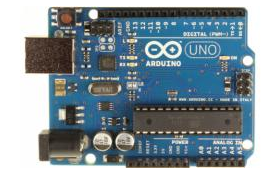
\includegraphics[width=1.0\linewidth]{ard_front.png}
\end{minipage}
\begin{minipage}[H]{.8\textwidth}
    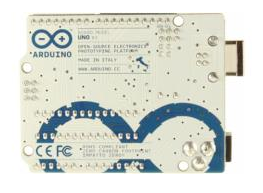
\includegraphics[width=1.0\linewidth]{ard_back.png}
\end{minipage}
\end{center}
\subsubsection{Opis}
Głową systemu  jest płytka arduino UNO R3.  Odpowiada za kolekcjonowanie częstotliowści z sensora i sterowanie serwami. Określa i przechowuje dane dotyczące kolorów i kątów kontenerów.
\subsubsection{Specyfikacja}
\begin{center}
\begin{tabular}{ | m{5cm} | m{3cm} | } 
\hline
Mikrokontroler&mikroczip ATmega328P\\
\hline
Napięcie wejściowe &  7-20 Volts\\ 
\hline
Napięcie operatywne &  5 Volts\\ 
\hline
\hline
Flash Memory& 32 KB\\
\hline
Piny Cyfrowe I/O & 14\\  
\hline
Piny Analogowe & 6\\ 
\hline
DC Current na I/O Pin& 20 mA\\ 
\hline
DC Current dla 3.3V Pin:& 50 mA\\ 
\hline
SRAM& 2 KB\\ 
\hline
EEPROM& 1 KB\\ 
\hline
Wysokość &  68.6 mm  \\ 
\hline
Szerokość &  53.4 mm \\ 
\hline
Waga &  25 g  \\ 
\hline
\end{tabular}
\end{center}
\subsection{Zasilacz}
\begin{center}
\begin{minipage}[H]{.85\textwidth}
    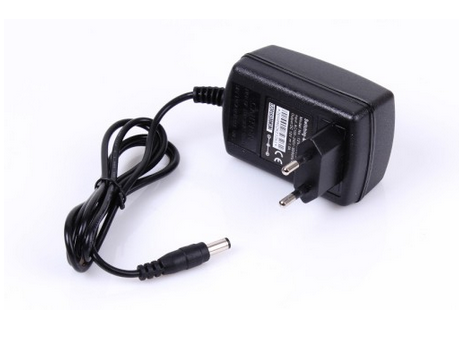
\includegraphics[width=1.0\linewidth]{zasilacz.png}
\end{minipage}
\end{center}
\subsubsection{Opis}
Dostarcza zasilanie dla całego systemu.
\subsubsection{Specyfikacja}
\begin{center}
\begin{tabular}{ | m{5cm} | m{3cm} | } 
\hline
Napięcie wyjściowe &  12 V\\ 
\hline
Napięcie zasilania & max 240 V\\ 
\hline
Prąd wyjściowy& 2 A\\
\hline 
\multicolumn{2}{|c|}{Wtyk DC}\\
\hline 
\multicolumn{2}{|c|}{Impulsowy}\\
\hline  
\multicolumn{2}{|c|}{Wtyczkowy}\\ 
\hline
\end{tabular}
\end{center}
\subsection{Włącznik/ Wyłącznik}
\begin{center}
\begin{minipage}[H]{.65\textwidth}
    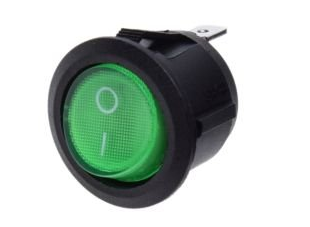
\includegraphics[width=1.0\linewidth]{switcher.png}
\end{minipage}
\end{center}
\subsubsection{Opis}
Pozwala na regulowanie dopływu prądu tzn, włączanie urządzenia oraz wyłączanie.
\subsubsection{Specyfikacja}
\begin{center}
\begin{tabular}{ | m{5cm} | m{3cm} | } 
\hline
Prąd& 6A \\
\hline
Napięcie& 230V\\
\hline
\end{tabular}
\end{center}
\subsubsection{Addytywnie kosztorys}
\begin{center}
\begin{tabular}{ | m{5cm} | m{3cm} | } 
\hline
Cena &  Komponent  \\
\hline
 2 zł & Włącznik \\
\hline
110 zł & Arduino Uno \\
\hline
15 zł & Serwo \\
\hline
30 zł & Kolor sensor \\
\hline
20 zł & Zasilacz\\
\hline


\end{tabular}
\end{center}

\end{document}
